\chapter{Numerical Solutions}
As we are interested in finding real valued solutions of our systems we also have to look into solving them numerically. This chapter focuses on the numerical solution of the mentioned systems.

We will first focus on methods used to solve a more general initial value problem of the form:

Find y, such that
\begin{align}
	\label{general numerical problem}
	y'(t) &= f(t,y), \quad t \in [t_0, t_l], \\
	y(t_0) &= y_0.
\end{align}

For this we presume that the function $f(t,y)$ is continuous and Lipschitz, we can apply the theorem of \emph{Picard-Lindelöf} \protecting{\cite[Satz~1.2.1]{NumerikGewöhnlicherDifferentialgleichungen}}, which states, that for every initial value $y_0$, the initial value problem \eqref{general numerical problem} is uniquely solvable in $[t_0, t_l]$.

In order to obtain an approximation to this unique solution we have to discretize. We first divide the time-intervall $[t_0, t_l]$ into
\begin{displaymath}
	t_0 < t_1 < ... < t_N \leq t_l
\end{displaymath}

and consider approximations $y_m \approx y(t_m)$ for $m=1,...,N$, see \ref{fig:numerical approximation}. We call this a \emph{time-grid} and we call the difference $h_{ij} = t_j - t_i$ with $0 \leq i < j \leq N$ the \emph{step size} from $t_i$ to $t_j$. We will only consider equidistant grids, i.e. $h_{ij} = h$ for all $0 \leq i,j \leq N$. A function defined on such a grid is called a \emph{grid-function}.

The grid function $y_h : T \to A$ with the time-grid $T={t_0, ..., t_N}$ and the approximated values $A = {y_0, ..., y_N}$ is called the \emph{numerical approximation} (of $y$ on the time grid).
\begin{figure}[H]
	\label{fig:numerical approximation}
	\centering
	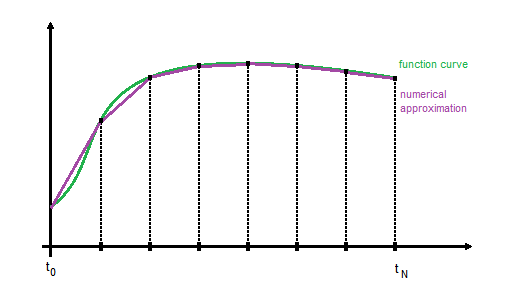
\includegraphics[scale=0.7]{pictures/num_approx.png}
	\caption{approximation of a function using numerical methods}
\end{figure}

\section{Single-Step-Methods}
	The first class of numerical methods we will consider are single-step methods. These methods use the previous approximated value $y_j$ and (for implicit methods) also the current approximated value $y_{j+1}$ to determine the current value $y_{j+1}$ through a \emph{procedural function}.
	
	\begin{definition}
		\label{def:single step mehod}
		A numerical method to approximate a differential equation \ref{general numerical problem} on a time-grid $t_0,...,t_l$ with the intermediate values $y_0,...,y_l$ is called a single-step method if it is of the form
		\begin{equation}
			\label{single-step method}
			y_{j+1} = y_j + h_j \phi(t_j,y_j, y_{j+1},h_j).
		\end{equation}
		We call $\phi$ the \emph{procedural function}. If $\phi$ does not depend on $y_{j+1}$, then the method is called \emph{explicit}, otherwise it is called \emph{implicit}.
	\end{definition}

	\subsection{Consistency, Stability and Convergence}
	
	In order to compare different single-step methods we have to define some notions to compare their quality. This leads to the definition of the error of the method, its consistency and its convergence. We begin with the definition of the error.
	
	\begin{definition}\label{Discretization_Error_SingleStep}
		Let $\tilde{y}_{m+1}$ be the result of one step of a single step method \eqref{single-step method} with the exact start-vector $y_m = y(t_m)$ then
		\begin{equation}
			\label{local discretization error single step}
			 \delta_{m+1} = \delta(t_m+h) = y(t_{m+1}) - \tilde{y}_{m+1}, \quad m = 0,...,N-1
		\end{equation}
		is called the \emph{local discretization error} of the single step method at the point $t_{m+1}$.
	\end{definition}

	The local error quantifies the error of every step of the method with respect to the exact solution. In most applications the exact solution is not known. Next we consider the consistency.

	\begin{definition}\label{Consistency_SingleStep}
		A single-step method is called \emph{consistent} if for all initial value problems \eqref{general numerical problem} 
		\begin{equation}
			\lim\limits_{h \to 0} \frac{\|\delta(t+h)\|}{h} = 0 \quad \text{for} \quad t_0 \leq t \leq t_l
		\end{equation}
		holds.\newline
		It is called \emph{consistent of order p}, if for a sufficiently smooth function $f$
		\begin{equation}
			\|\delta(t+h)\| \leq Ch^{p+1} \quad \text{for all} \quad h \in \mathopen{(} 0,H \mathclose{]} \quad \text{and} \quad t_0 \leq t \leq t_l - h
		\end{equation}
		holds with $C$ independent of $h$.
	\end{definition}

	Consistency aims to give insight in how similar the problem \eqref{single-step method} that the numerical method solves is to the real problem \eqref{general numerical problem}. Finally we consider convergence of a single step method \ref{def:single step mehod}.

	\begin{definition}\label{Convergence_SingleStep}
		A single-step method is called \emph{convergent}, if for all initial value problems \eqref{general numerical problem} for the \emph{global discretization error}
		\begin{displaymath}
			e_m = y(t_m)-y_m
		\end{displaymath}
		holds that
		\begin{displaymath}
			\max\limits_{m}\|e_m\| \to 0 \quad \text{for} \quad h_{max} \to 0.
		\end{displaymath}
		The single-step method is called to have the \emph{convergence order} $p$, if
		\begin{displaymath}
			\max\limits_{m} \|e_m\| \leq C h_{max}^p \quad \text{for} \quad h_{max} \in \mathopen{(} 0,H \mathclose{]} \quad \text{with} \quad t_0 \leq t_m \leq t_l
		\end{displaymath}
		with the constant $C$ not dependent on the step size $h$.
	\end{definition}

	As the name suggestes convergence tries to quantify how far off a numerical solution is from the real solution of a system. A very interesting result follows if we additionally require the single-step method to be stable.
	
	\begin{definition}\label{Discrete_Stability_SingleStep - lecture notes for numpdgl}
		A single-step method is called \emph{(discretely) stable} if for grid-functions $y_h$ and $\tilde{y}_h$ with
		\begin{align}
			y_{i+1} &= y_i + h \phi(t_i, y_i), \\
			\tilde{y}_{i+1} &=  \tilde{y}_i + h [\phi(t_i, \tilde{y}_i) + \theta_i],
		\end{align}
		and perturbations $\theta_i = \theta_h(t_i)$ of the right side as well as a bounded perturbation in the initial-values $y_0 - \tilde{y}_0$ the error is bounded by
		\begin{displaymath}
			\|y_h - \tilde{y}_h\|_{\infty,h} \leq C (\|y_0 - \tilde{y}_0\|_{l^2} + \|\theta_h\|_{\infty,h})
		\end{displaymath}
		with a constant $C$ which is not dependent on $h$. The norm $\|.\|_{\infty,h}$ denotes the maximum norm over the time-grid, i.e. for a function $b: T={t_0,...,t_N} \to \mathbb{R}^d$ we have $\|b\|_{\infty,h} = \max\limits_{t \in T}\|b(t)\|$, $\|b\|$ is the euclidean norm.
	\end{definition}
	
	For single-step methods which are consistent and stable we obtain the following convergence theorem.
	
	\begin{theorem}[Lax-Richtmyer]\label{Lax-Richtmyer}
		A consistent (with order $p$) and discretely stable single-step method is convergent (with order $p$).
	\end{theorem}
	
	This theorem is due to Lax and Richtmyer. The converse of this statement is also true. 

	\subsection{further stability properties}
		from numpdgl skript \\
		In this section we consider as a model problem the Dahlquist equation, i.e. find $u$ such that
		\begin{align}
			u' &= \lambda u, \quad t > 0 \\
			u(0) &= u_0
		\end{align}
		with $\lambda \in \mathbb{C}$ and $u_0$ fixed.
		
		\begin{definition}
			\begin{enumerate}
				\item 
				If a single-step method can be written in the form
				\begin{equation}
					u_{i+1} = R(z) \ u_i, \quad z:= h \ y
				\end{equation}
				then we call $R: \mathbb{C} \to \mathbb{C}$ the \emph{stability function} of the single-step method.
				\item 
				The set
				\begin{equation}
					S := \{z \in \mathbb{C} : |R(z)| \leq 1\}
				\end{equation}
				is called the \emph{region of stability} of the method.
				\item 
				A single-step method is called
				\begin{itemize}
					\item \emph{0-stable}, if $0 \in S$.
					\item \emph{A-stable}, if $\mathbb{C}^- \subset S$.
					\item \emph{L-stable}, if $R(z) \to 0$ for $Re(z) \to -\infty$.
				\end{itemize}
			\end{enumerate}
		\end{definition}

	%\subsection{Runge-Kutta Methods}
	%	A very prevalent family of numerical single-step methods are the \emph{Runge-Kutta} methods. 
		
		%\begin{figure}
		%	\centering
		%	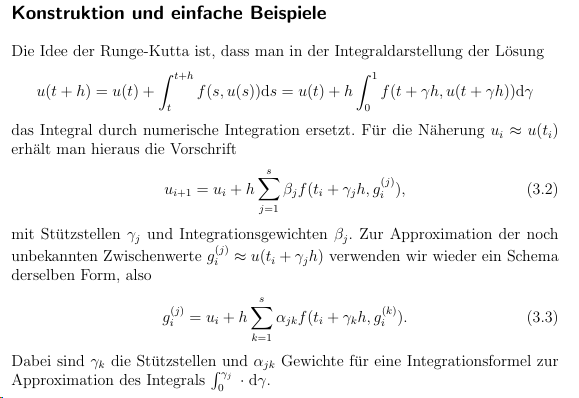
\includegraphics[width=0.7\linewidth]{screenshot026}
		%	\caption{}
		%	\label{fig:screenshot026}
		%\end{figure}
		
	%	\begin{definition}
	%		Let $s \in \mathbb{N}$. A single-step method of the form
	%		\begin{align}
	%			y_{m+1} = y_m + h \sum_{i=1}^{s} b_i f(t_m + c_ih, y_{m+1}^{(i)}) \\ 
	%			y_{m+1}^{(i)} = y_m +  \sum_{j=1}^{s} a_{ij} f(t_m + c_jh, y_{m+1}^{(j)})
	%		\end{align}
	%		is called a \emph{Runge-Kutta Method} with $s$ steps.
	%	\end{definition}
		
	%	We usually collect the coefficients into the vectors and matrices $c=(c_1, ...,c_s)$, $A = (a_{ij})_{ij}$ and $b=(b_1, ..., b_s)$.
		
	%	If $A$ is a strictly lower triangle matrix, this means for all $j \geq i$ holds $a_{ij} = 0$ then the Runge-Kutta method is explicit, otherwise it is implicit. In general implicit Runge-Kutta methods might need more computational effort because to calculate $y_m^{(i)}$ a nonlinear system of equations has to be solved. But in contrast those methods can also lead to very good stability characteristics.
		
	%	\begin{lemma}\cite{NumerikGewöhnlicherDifferentialgleichungen}
	%		A Runge-Kutta mehtod is consistent, if and only if
	%		\begin{displaymath}
	%			\sum_{i=1}^{s} b_i = 1
	%		\end{displaymath}
	%	\end{lemma}
	
	%	The coefficients of a Runge-Kutta method are usually represented in the \emph{Butchertableau}, which was introduced by John C. Butcher and has the following form.
		
	%	\begin{displaymath}
	%		\begin{array}{c|ccc}
	%			c_1 & a_{11} & \dots & a_{1s} \\
	%			\vdots & \vdots & & \vdots \\
	%			c_s & a_{s1} & \dots & a_{ss} \\
	%			\hline
	%			 & b_1 & \dots & b_s
	%		\end{array}
	%		\qquad
	%		\text{of in matrix form}
	%		\qquad
	%		\begin{array}{c|c}
	%			c & A \\
	%			\hline
	%			 & b
	%		\end{array}
	%	\end{displaymath}
	
	%	Their stability can directly be derived from the butcher tableau. The stability function of an arbitrary m-stage Runge-Kutta method has the form
	%	\begin{displaymath}
	%		R(z) = 1+zb^\top (I_m-zA)^{-1}e
	%	\end{displaymath}
	
	%	where $e = (1,...,1)$.
		
	%	\textbf{Remark:} The trapezoidal rule is a widely used Runge-Kutta method which we can also consider as a multistep-method. It will be discussed later on.
	
			
\section{Multistep-Methods}
	based on chapter 4 of book num gew dgl steif nichtsteif \newline
	Linear multistep methods (LMSM) use approximations $u_{m+l}$ along the gridpoints $t_{m+l}, \quad l=0,1,...,k-1$ to calculate the new approximation $u_{m+k}$ at $t_{m+k}$. We will first discuss topics related to the order of the methods depending on its parameters, stability and convergence.
	
	\begin{definition}
		\label{def:multi step method}
		For given $\alpha_0, ..., \alpha_k$ and $\beta_0, ..., \beta_k$ the iteration rule
		\begin{equation}
			\label{linear-multistep-method}
			\sum_{l=0}^{k} \alpha_l u_{m+l} = h \sum_{l=0}^{k} \beta_l f(t_{m+l}, u_{m+l}), \quad m=0,1,...,N-k
		\end{equation}
		is called a \emph{linear multistep method} (linear k-step method). It is always assumed that $\alpha_k \neq 0$ and $|\alpha_0| + |\beta_k| > 0$. If $\beta_k=0$ holds, then the method is called explicit, otherwise implicit.
	\end{definition}
	
	A linear multi-step method consists of two parts:
	\begin{enumerate}
		\item In the \emph{starting-phase} approximations $u_1,...,u_{k-1}$ for the first $k-1$ gridpoints $t_l = t_0+th, l=1,...,k-1$ have to be calculated. For example we can use aa single-step method or a multi-step method with fewer steps.
		
		\item  In the \emph{run-phase} the multi-step formula is used to determine new approximations $u_{m+k}$ for the gridpoint $t_{m+k}$
	\end{enumerate}
	
	For theoretical analysis of the multi-step methods we consider the generating polynomials of a multi-step method \ref{def:multi step method}.
	\begin{equation}
		\label{eq:generating polynomials multistep method}
		\rho(x) := \sum_{l=0}^{k} \alpha_l x^l
		\qquad \text{and} \qquad
		\sigma(x) := \sum_{l=0}^{k} \beta_l x^l
	\end{equation}
			
	
	\subsection{Consistency, Stability and Convergence}
	\cite{NumerikGewöhnlicherDifferentialgleichungen}
	
	Again we need to define the properties consistency, stability and convergence for this method.
	\begin{definition}
		Let $\tilde{y}_{m+k}$ be the result of one step of the multi-step method \eqref{linear-multistep-method} with the start-values given as the evaluations of the exact solution $y_{m+l} = y(t_{m+l})$ at $0 \leq l < k$. This means
		\begin{displaymath}
			\alpha_k \tilde{u}_{m+k} = \sum_{l=0}^{k-1} \left( h \beta_l f(t_{m+l}, y(t_{m+l})) - \alpha_l y(t_{m+l}) \right) + h \beta_k f(t_{m+k}, \tilde{u}_{m+k}) .
		\end{displaymath}
		Then
		\begin{displaymath}
			\delta_{m+k} = \delta(t_{m+k}) = y(t_{m+k}) - \tilde{u}_{m+k}, \quad m=0,1,...,N-k
		\end{displaymath}
		is called the \emph{local discretization error} (local error) of the linear multi-step method, see Def. \ref{linear-multistep-method} at the point $t_{m+k}$.
	\end{definition}
	
	For $k=1$ this definition agrees with the definition of the local discretization error for single-step methods \ref{Discretization_Error_SingleStep}.
	If we assign the difference operator
	\begin{equation}
		L[y(t),h] = \sum_{l=0}^{k} \left( \alpha_l y(t+lh) - h \beta_l y'(t+lh) \right)
	\end{equation}
	to the linear mutli-step method, we gain the following definition for consistency of such a methods.
	
	\begin{definition}
		A linear multi-step method is called %\emph{preconsistent} if for all functions $y(t) \in C^1[t_0,t_l]$
%		\begin{displaymath}
%			\lim\limits_{h \to 0} L[y(t),h]=0
%		\end{displaymath}
%		holds. 
%		It is called 
		\emph{consistent}, if for all functions $y(t) \in C^2([t_0,t_l])$
		\begin{displaymath}
			\lim\limits_{h \to 0} \frac{1}{h} L[y(t),h] = 0
		\end{displaymath}
		holds. It has the \emph{consistency order p}, if for all functions $y(t) \in C^{p+1}[t_0, t_l]$
		\begin{displaymath}
			L[y(t),h] = \mathcal{O}(h^{p+1}) \quad \text{for} \quad h \to 0
		\end{displaymath}
		holds.
	\end{definition}

	From the generating polynomials \eqref{eq:generating polynomials multistep method} we can derive simple consistency conditions, i.e.
	\begin{displaymath}
		\rho(1) = 0 \quad \text{and} \quad \rho'(1) = \sigma(1).
	\end{displaymath}

	Next we also need convergence of such methods.
	
	\begin{definition} \label{def: LMSM convergence}
		We say that a linear multi-step method is convergent if for a solution $y$ of the problem a solution vector created by an LMSM $y_j$ for $j \in {0,...,k}$ we have that
		\begin{displaymath}
			\lim\limits_{h \to \infty} \max_{0 \leq j \leq k} ||y(t_j) - y_j|| = 0.
		\end{displaymath}
	\end{definition}
	
	%\begin{figure}
	%	\centering
	%	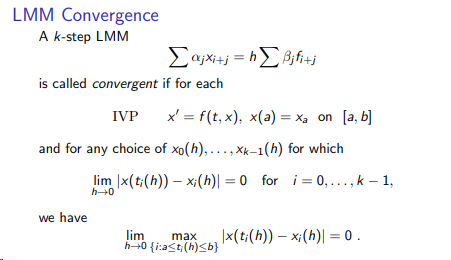
\includegraphics[width=0.7\linewidth]{screenshot025}
	%	\caption{}
	%	\label{fig:screenshot025}
	%\end{figure}
	
	The discrete stability is also very similar to the single-step methods.
	\begin{definition} \label{discrete stability LMSM}
		A linear multi-step method is called (discretely) stable, if for solutions $u_h$ and $\tilde{u}_h$ of
		\begin{align}
			\sum_{l=0}^{k} \alpha_l u_{m+l} &= h \sum_{l=0}^{k} \beta_l f(t_{m+l}, u_{m+l}), \\
			\sum_{l=0}^{k} \alpha_l \tilde{u}_{m+l} &= h \sum_{l=0}^{k} \beta_l f(t_{m+l}, \tilde{u}_{m+l}) + h\theta_n
		\end{align} 
		and bounded initial values $y_j - \tilde{y}_j$ for $j \in {0,...,k}$ we have that
		\begin{displaymath}
			\max_{t_0 \leq t_n \leq T} ||y_n - \tilde{y}_n|| \leq C \sum_{j=0}^{k-1} ||y_j - \tilde{y}_j|| + \max_{t_0 \leq t_n \leq T} ||\theta_n||.
		\end{displaymath}
	\end{definition}
	
%	\begin{definition}
%		A linear multi-step method is called \emph{zero-stable} if all solutions of the difference equation
%		\begin{displaymath}
%			\sum_{l=0}^{k} \alpha_l u_{m+l} = 0
%		\end{displaymath}
%		are bounded.
%	\end{definition}
	
%	\textbf{Lax-Richtmyer}
	
%	\begin{theorem}
%		A linear multi-step method is zero-stable, if and only if the polynomial $\rho(x)$ fullfills the ``root-condition'', this means:
%		\begin{enumerate}
%			\item All roots $\bar{x}$ of $\rho(x)$ are within the unit-circle $|\bar{x}| \leq$ in the complex plane.
%			\item All roots $\bar{x}$ with $|x| = 1$ are singular.
%		\end{enumerate}
%	\end{theorem}
	
%	\begin{theorem}%[DAE lecture]
%		A linear multistep method is stable if and only if it is zero-stable.
%	\end{theorem}
	
	%\textbf{from circuit book below, above from modelling book}
	
	\subsection{further stability properties}
	
	In this section we consider again the Dahlquist test problem as a model problem
	\begin{align}
		u' &= \lambda u, \quad t > 0 \\
		u(0) &= u_0
	\end{align}
	with $\lambda \in \mathbb{C}$ and $u_0$ fixed.\\
	
	%Asessment for stiff equations lt wikipedia (LMSM)
	
	Thus the resulting linear multistep method is of the form
	\begin{align*}
		\sum_{l=0}^{k} \alpha_l u_{n+l} = h \sum_{l=0}^{k} \beta_l \lambda u_{n+l} \\
		\iff \sum_{l=0}^{k}  [\alpha_l - h \beta_l \lambda] u_{n+l}
	\end{align*}
	
	%in numerik book auf seite 326
	
	Using this we define the following important stability notions.
	\begin{definition}
		\begin{enumerate}
			\item 
			The set
			\begin{equation}
				\begin{aligned}
					S := \{z \in \mathbb{C} : \rho(\xi) - z \sigma(\xi) = 0 \implies \xi \in \mathbb{C} \text{ and } |\xi| \leq 1. \\
					\text{ If $\xi$ has multiplicity greater than $1$, then } |\xi| < 1\}
				\end{aligned}
			\end{equation}
			is called the region of stability of the method.
			\item 
			A linear multistep method is called
			\begin{itemize}
				\item \emph{0-stable}, if $0 \in S$.
				\item stable in the point $z \in \mathbb{C}$, if $z \in S$.
				\item \emph{$A(\alpha)$-stable}, if it is stable in all $z$ that lie within the set $\{z \in \mathbb{C}^- : |arg(z)-\pi| \leq \alpha\}$ for $\alpha \in (0, \frac{\pi}{2})$.		 
			\end{itemize}
		\end{enumerate}
	\end{definition}
	
	seite 314 im buch numerik 
	
	\begin{figure}[H]
		\centering
		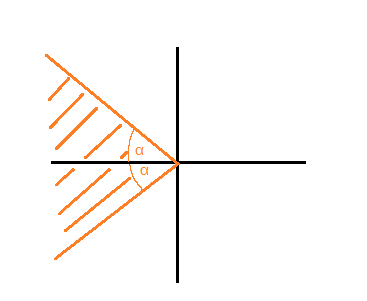
\includegraphics[width=0.3\linewidth]{screenshot021}
		\caption{$A(\alpha)$ stability for $\alpha = \frac{\pi}{4}$}
		\label{fig:screenshot021}
	\end{figure}
	
	following from numerik buch seite 134
	\begin{theorem}[\protecting{\cite[Satz~4.2.10]{NumerikGewöhnlicherDifferentialgleichungen}}]
		\label{th: null-stbaility and consistence is convergence}
		Let $f(t,y)$ be sufficiently smooth and the linear multi-step method be zero-stable and consistent of order $p$, then it is also convergent of order $p$.
	\end{theorem}
	
	equivalent to lax richtmyer in single step because for lmsm zero stable = stable
	

\section{Implicit linear multi-step formulas}
These kinds of multi-step methods are commonly used to numerically solve the systems obtained using modified nodal analysis.
%Our assumption that we only consider network equations arising from networks consisting of RLC components as well as controlled sources which keep the index between 1 and 2 still holds.

What equations do we consider?

%We consider the equations in charge/flux oriented formulation introduced in section \ref{sec:charge flux oriented formulation}
%\begin{align*}
%	0 &=
%	\underbrace{ 
%	\left( \begin{matrix}
%		A_c & 0 \\
%		0 & I \\
%		0 & 0
%	\end{matrix} \right)}_{=:A}
%	\underbrace{
%	\left( \begin{matrix}
%		q' \\
%		\phi'
%	\end{matrix} \right)}_{=:y'}
%	+
%	\underbrace{
%	\left( \begin{matrix}
%		A_R r(A_R^\top u,t) + A_L i_L + A_V i_V + A_I i(u, i_L, i_V, t) \\
%		- A_L^\top u \\
%		v(u, i_L, i_V, t) - A_V^\top u
%	\end{matrix} \right)}_{=:f(x,t)}, \\
%	\underbrace{
%	\left( \begin{matrix}
%		q \\
%		\phi 
%	\end{matrix} \right)}_{=:y} 
%	&=
%	\underbrace{
%	\left( \begin{matrix}
%		q_C(A_C^\top u) \\
%		\phi_L(i_L) 
%	\end{matrix} \right)}_{=:g(x,t)},
%\end{align*}
%
%or simply
%\begin{align*}
%	0 &= F(y'(t), x(t), t) :=A y'(t) + f(x(t),t), \\
%	0 &= y(t) - g(x(t)).
%\end{align*}
%with the unknowns $x:=(u, i_L, i_V)^\top$.

The approach to solve those systems numerically can be split into three main steps:
\begin{enumerate}
	\item Computation of consistent initial values
	
	The first step is to compute consistent inital values $(x_0, y_0)$ at the initial time point $t_0$. In the index-1 case this can be done by solving a so called steady state problem. Steady state means that we consider a time-independent circuit (DC operating point). This means we have to solve
	\begin{displaymath}
		F(0,x_0,t_0) = 0
	\end{displaymath}
	
	for $x_0$ and then set $y_0 = g(x_0)$.
	
	\item Numerical integration based on multi-step schemes
	
	Using the consistent initial values, we obtain solutions of the network equations at discrete timepoints $t_1, t_2, ...$ by integration with linear multi-step methods.
\end{enumerate}

In the following two subchapters we will give a short overview over the two most commonly used methods for solving these kinds of systems.

\subsection{BDF-k methods}
	\label{ch:BDf-k methods}
	chapter 9.2 numerik book
	wikipedia
	
	The most commonly used numerical methods for solving the systems that arise in electrical circuits are the BDF-scheme and the trapezoidal rule. 
	
	We will not give a deeper look into their construction but will only state their properties. BDF schemes are appealing because they save function evaluations as much as possible, since this is very costly in circuit simulation.
	
	The \emph{backward differentiation formula (BDF)} is a family of implicit linear multistep methods. They have the general form
	\begin{equation}
		\sum_{k=0}^{s} \alpha_k y_{n+k} = h \beta f(t_{n+s}, y_{n+s})
	\end{equation}

	Since we are interested in the unknown $y_{n+s}$ which is used to evaluate $f$, this method is implicit. The coefficients $\alpha_k$ and $\beta$ are chosen, such that the method achieves the best possible order $s$.
	
	The BDF or BDF-k formulas for $k=1,...,3$ have the following form %or till 6
	\begin{align*}
		k = 1 &: h f_{m+1} = u_{m+1} - u_m \\
		k = 2 &: h f_{m+2} = \frac{1}{2} (3 u_{m+2} - 4 u_{m+1} + u_m) \\
		k = 3 &: h f_{m+3} = \frac{1}{6} (11 u_{m+3} - 18 u_{m+2} + 9 u_{m+1} - 2 u_m) %\\
%		k = 4 &: h f_{m+4} = \frac{1}{12} (25 u_{m+4} - 48 u_{m+3} + 36 u_{m+2} - 16 u_{m+1} + 3 u_m) \\
%		k = 5 &: h f_{m+5} = \frac{1}{260} (137 u_{m+5} - 300 u_{m+4} + 300 u_{m+3} - 200 u_{m+2} +75 u_{m+1} -12 u_m) \\
%		k = 6 &: h f_{m+6} = \frac{1}{60} (147 u_{m+6} - 360 u_{m+5} + 450 u_{m+4} - 400 u_{m+3} + 225 u_{m+2} - 72 u_{m+1} + 10 u_m)
	\end{align*}
	
	Methods with $k > 6$ are not zero-stable. Indeed in practice, methods with order greater than 3 are rarely used because of their stability properties. The stability-region shrinks with increasing order.
	
	BDF schemes have consistency order $p = k$. They are methods for solving stiff equations, thus their stability is indicated by their region of absolute stability. Unfortunately not all BDF-schemes are A-stable, but their stability region still contains a large part of the complex left half-plane, see Figure \ref{fig:screenshot020} They are the most efficient linear multistep methods of this kind.
	
	\begin{figure}[H]
		\centering
		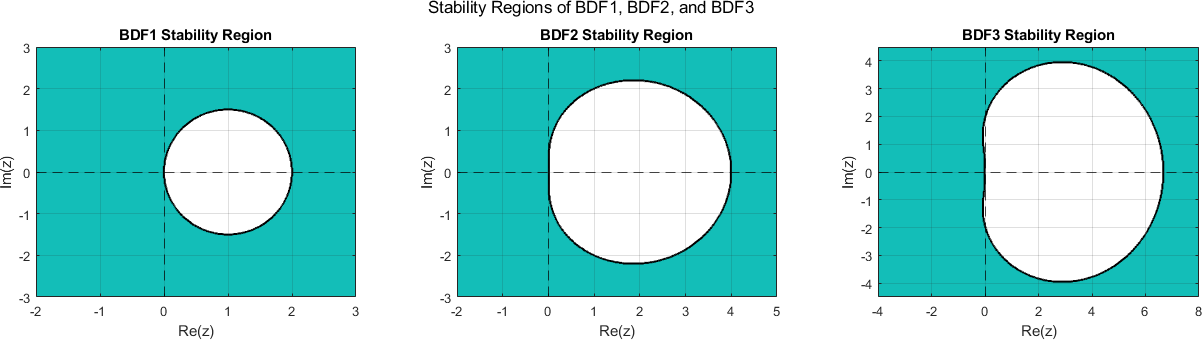
\includegraphics[width=1\linewidth]{pictures/bdf_stability_regions.png}
		\caption{stability regions of BDF-schemes}
		\label{fig:screenshot020}
	\end{figure}
	
	The first timestep is always performed by BDF1 (implicit Euler scheme) as a starting procedure. sure? not really
	
	The Order of consistency of this family of multi-step methods is given by the following theorem
	
	\begin{theorem}[\protecting{\cite[Satz~9.2.1]{NumerikGewöhnlicherDifferentialgleichungen}}]
		The BDF-k methods have consistency order $p=k$.
	\end{theorem}
	
	Due to Theorem \ref{th: null-stbaility and consistence is convergence} and the fact that BDF-k methods are $0$-stable, they are also convergent with order k.
	
	Seite 106 numerik - schrittweite für startwerte bei bdf3 kleiner für kleineren fehler, halbieren, vierteln, achteln whatever
	
\subsection{trapezoidal rule}
	\label{ch:trapezoidal rule}
	
	The trapezoidal rule is a natural alternative to BDF2 since it is A-stable and a linear multistep method of order 2 the one with the smallest leading error coefficient. (\cite{ModellingAndDiscretizationOfCircuitProblems})
	
	It works by approximating the region under the graph of the function $f(x)$ as a trapezoid, hence the name. It follows that	
	\begin{displaymath}
		\int_{a}^{b} f(x) dx \approx (b-a)\frac{1}{2} (f(a)+f(b))
	\end{displaymath}
	
	This procedure is repeated for small subsections of the intervall $[a,b]$. Thus we obtain the iteration formula
	\begin{displaymath}
		u_h (t+h) = u_h(t) +\frac{h}{2}[f(t,u_h(t)) + f(t+h, u_h(t+h))].
	\end{displaymath}
%	
%	This iteration rule can also be formulated using the butcher tableau	
%	\begin{displaymath}
%		\begin{array}{c|cc}
%			0 & 0 & 0 \\
%			1 & \frac{1}{2} & \frac{1}{2} \\
%			\hline
%			& \frac{1}{2} & \frac{1}{2}
%		\end{array}
%	\end{displaymath}
	
	Because $u_h(t+h)$ appears in $f$ again we see that this is an implicit method. %The butcher tableau confirms this as well.
	
\section{Numerical Examples}
	
	In this section we will apply the Trapezoidal rule as well as the BDF-k schemes for our three examples (reference!!!!!!!!!).
	
	
	\textbf{Example 1} \\
		
	\begin{figure}[H]
		\centering
		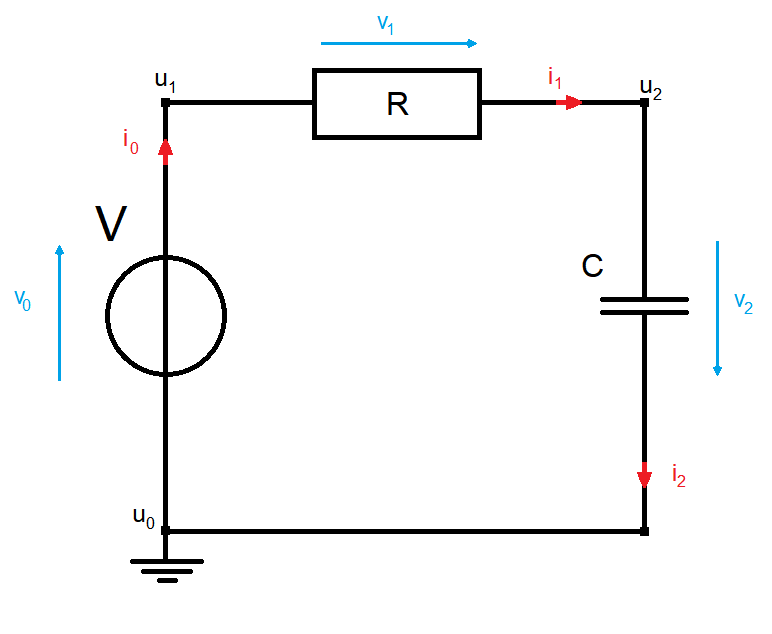
\includegraphics[scale=0.4]{pictures/Example1_simple_p2.png}
		\caption{charging capacitor with series resistor and voltage source}
	\end{figure}
	
	The MNA-system for this example reads as
	
	\begin{equation}
		\label{eq:MNA-system of chargin capacitor}
		\begin{pmatrix}
			0 & 0 & 0 \\
			0 & C & 0 \\
			0 & 0 & 0
		\end{pmatrix}
		*
		\begin{pmatrix}
			u_,' \\
			u_2' \\
			i_0'
		\end{pmatrix}
		+
		\begin{pmatrix}
			\frac{1}{R} & \frac{1}{R} & 0 \\
			\frac{1}{R} & \frac{1}{R} & -1 \\
			0 & -1 & 0 
		\end{pmatrix}
		*
		\begin{pmatrix}
			u_1 \\
			u_2 \\
			i_0
		\end{pmatrix}
		=
		\begin{pmatrix}
			0 \\
			0 \\
			-v_{src}
		\end{pmatrix}.
	\end{equation}

	For testing we set the resistance to $R=1$ and the capacitance to $C=1$. In our case we let the  voltage source supply a voltage of the form $v_{src} = sin(\pi t)$.
	
	\begin{center}
		\begin{tabular}{ c || c c c | c c c | c c c | } 
			h & \multicolumn{3}{c|}{k = 1} & \multicolumn{3}{c|}{k = 2} & \multicolumn{3}{c|}{k = 3} \\
			 & u1 & u2 & iL & u1 & u2 & iL & u1 & u2 & iL \\
			\hline
			 & \multicolumn{3}{c|}{Error} & \multicolumn{3}{c|}{Error} & \multicolumn{3}{c|}{Error} \\
			\hline
			1 & number & number & number & number & number & number & number & number & number \\
			0,1 & number & number & number & number & number & number & number & number & number \\
			0,01 & number & number & number & number & number & number & number & number & number
		\end{tabular}
	\end{center}


	\textbf{Example 2} \\
	
	\begin{figure}[H]
		\centering
		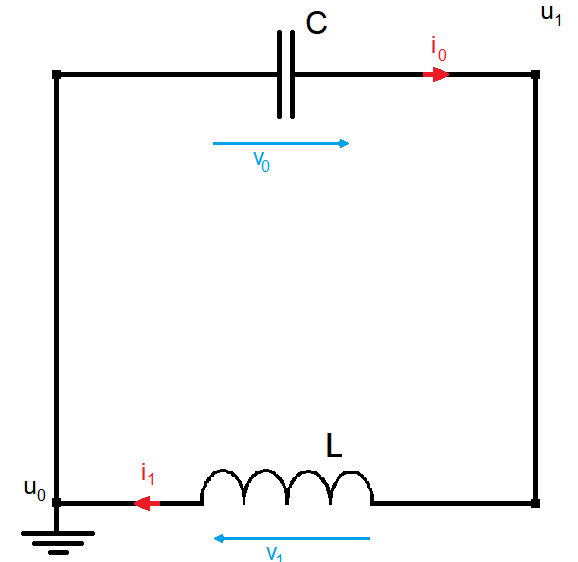
\includegraphics[scale=0.4]{pictures/Example2_index0.png}
		\caption{LC-circuit}
	\end{figure}

	The MNA-system for this example reads as
	
	For testing we set the capacitance to $C=1$ and the inductance to $L=1$.
	
	With the initial conditions $u_1(0) = 1$ and $i_L(0) = 0$, the exact solutions for the voltage $u_1$ and the current $i_L$ then have the form \ref{fig: Exact solution for example 2}.	
	
	\begin{figure}[H]
		\label{fig: Exact solution for example 2}
		\centering
		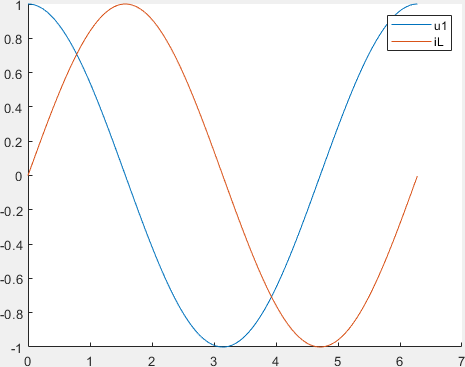
\includegraphics[scale=0.7]{pictures/exact_solution_ex2.png}
		\caption{Exact solution for example 2.}
	\end{figure}
	
	Applying the BDF-k methods \ref{ch:BDf-k methods} and the Trapezoidal rule \ref{ch:trapezoidal rule} to this problem we can observe the maximal error $err = \max\limits_{0 \leq t \leq T} \| y(t) - \tilde{y}(t) \|$. This error is displayed in table \ref{tab:error ex2}.
	
	
	\begin{table}[H]
		\resizebox*{\textwidth}{!}{%
			\csvreader[tabular= | c || c c | c c | c c | c c | ,
			table head = \hline h & \multicolumn{2}{c|}{k = 1} & \multicolumn{2}{c|}{k = 2} & \multicolumn{2}{c|}{k = 3} & \multicolumn{2}{c|}{Trapezoidal} \\
			& u1 & iL & u1 & iL & u1 & iL & u1 & iL \\
			\hline,
			late after line=\\\hline]
			{../Matlab/err_ex2.csv}{h=\h, oneu=\oneu, onei=\onei, twou=\twou, twoi=\twoi, threeu=\threeu, threei=\threei, trapu=\trapu, trapil=\trapil}
			{\h & \num{\oneu} & \num{\onei} & \num{\twou} & \num{\twoi} & \num{\threeu} & \num{\threei} & \num{\trapu} & \num{\trapil}}
		}
	\end{table}
	
%	\begin{table}[H]
%	\begin{center}
%		\label{tab:error ex2}
%		\begin{tabular}{ c || c c | c c | c c | c c |} 
%			h & \multicolumn{2}{c|}{k = 1} & \multicolumn{2}{c|}{k = 2} & \multicolumn{2}{c|}{k = 3} & \multicolumn{2}{c|}{Trapezoidal} \\
%			& u1 & iL & u1 & iL & u1 & iL & u1 & iL \\
%			\hline
%			& \multicolumn{2}{c|}{err x e-1} & \multicolumn{2}{c|}{err x e-3} & \multicolumn{2}{c|}{err x e-4} & \multicolumn{2}{c|}{err x e-3} \\
%			\hline
%			$1$ & $0,1$ & $0,1$ & $1180$ & $1220$ & $25100$ & $22000$ & $1390$ & $1460$ \\
%			$0,1$ & $7,14$ & $6,90$ & $78,3$ & $80,2$ & $639$ & $615$ & $19,6$ &  $20,8$ \\
%			$0,01$ & $1,18$ & $1,11$ & $0,79$ & $0,83$ & $0,68$ & $0,63$ & $0,19$ & $0,20$
%		\end{tabular}
%		\caption{Error for BDF-1, -2, -3 methods and trapezoidal rule applied to ex2.}
%	\end{center}
%	\end{table}

	By comparing the errors of the methods we can see that they indeed have the predicted convergence order. (reference appropriate theorems here)

	\textbf{Example 3} \\
	
	\begin{figure}[H]
		\centering
		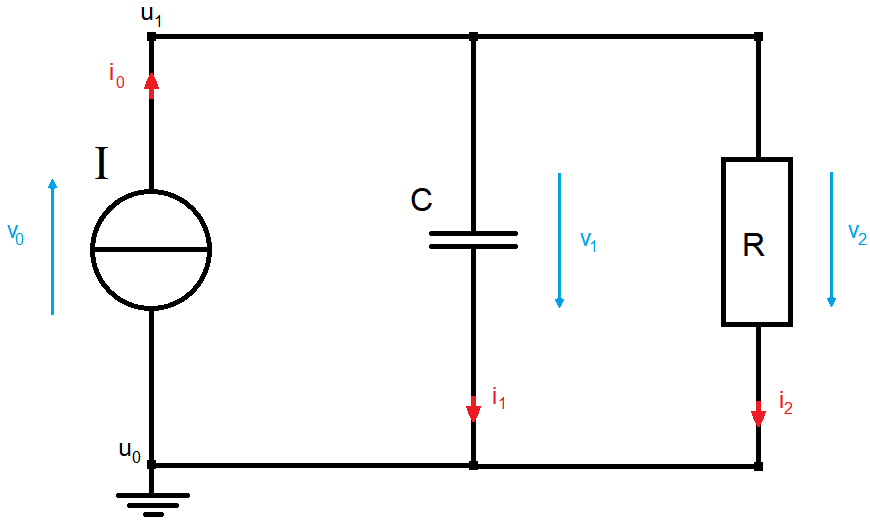
\includegraphics[scale=0.4]{pictures/Example3.png}
		\caption{Current source with capacitor and resistor.}
	\end{figure}
	
	\begin{center}
		\begin{tabular}{ c || c c c | c c c | c c c | } 
			h & \multicolumn{3}{c|}{k = 1} & \multicolumn{3}{c|}{k = 2} & \multicolumn{3}{c|}{k = 3} \\
			& u1 & u2 & iL & u1 & u2 & iL & u1 & u2 & iL \\
			\hline
			& \multicolumn{3}{c|}{Error} & \multicolumn{3}{c|}{Error} & \multicolumn{3}{c|}{Error} \\
			\hline
			1 & number & number & number & number & number & number & number & number & number \\
			0,1 & number & number & number & number & number & number & number & number & number \\
			0,01 & number & number & number & number & number & number & number & number & number
		\end{tabular}
	\end{center}